\documentclass{ieeeaccess}
\usepackage{graphicx}
\usepackage{amsmath}
\usepackage{cite}
\usepackage{url}
\usepackage{array}
\newcolumntype{L}[1]{>{\raggedright\arraybackslash}p{#1}}
\setlength{\tabcolsep}{4pt}
\graphicspath{{figures/}}
\newcommand{\code}[1]{\texttt{#1}}
\newcommand{\degc}{\,^{\circ}\mathrm{C}}
\setlength{\emergencystretch}{1em}

\begin{document}
\history{AST01.41 Capstone Project Final Manuscript}
\title{PlantCare IoT for Soil Wetness and Thermal Exposure Monitoring in Potted Plants}
\author{\uppercase{Jirapat Datephanyawat and Waranon Neamtuptim}}
\address{ICT Department, School of Engineering and Technology, Asian Institute of Technology, Pathum Thani, Thailand}
\tfootnote{This work was carried out for AST01.41 Fundamentals of Internet of Things and Cloud Computing at the Asian Institute of Technology.}
\markboth{Datephanyawat and Neamtuptim: PlantCare IoT}{Datephanyawat and Neamtuptim: PlantCare IoT}

\begin{abstract}
Watering a potted plant on a fixed schedule can waste water or leave the root zone dry because the soil surface gives limited information about conditions below it. Uneven radiant heating adds a second condition that visual inspection can miss. A cloud-only monitor makes every reading depend on the uplink and has little reason to transmit every thermal frame at the local sampling rate. PlantCare IoT combines a capacitive probe and an eight-by-eight infrared array with an ESP32 that smooths soil readings, calculates a relative wetness index, and presents local readings. The firmware sends periodic HTTPS snapshots to Node-RED. InfluxDB and Grafana on the lab platform support time-series storage, historical review, and experimental status indicators. A saved Grafana Explore CSV contained 5,860 unique minute rows, of which 5,844 contained both soil and thermal fields. The export contained long gaps, including a 967-minute interval between consecutive rows. Four watering observations showed a consistent decrease in the raw soil reading immediately after watering. The prototype demonstrates a monitoring workflow with manual plant care. Its thresholds are specific to the trial, and controlled measurements of water savings, latency, link overhead, and energy efficiency remain outstanding.
\end{abstract}

\begin{keywords}
Edge computing, Internet of Things, soil wetness, thermal monitoring, time-series databases
\end{keywords}
\titlepgskip=-21pt
\maketitle

\section{Introduction, Problem Statement and Objectives}
\PARstart{W}{atering} a container plant requires judging the condition at the probe depth and interpreting how it changes after watering. A pot may look dry at the surface while deeper soil still holds water. Conversely, a fixed schedule may miss rapid drying near a sunlit opening. FAO AQUASTAT attributes about 69\% of global freshwater withdrawals to agriculture \cite{fao}. That context motivates measurement-informed water use, although the trial concerns a single pot and measures neither total irrigation volume nor water savings. Prior experiments with low-cost capacitive probes show the importance of soil-specific calibration \cite{calibration}. PlantCare therefore reports a relative index referenced to observations from its own pot.

The monitored plant was identified as \textit{Portulaca} in the firmware and local dashboard. The prototype follows changes in soil readings and uses a low-resolution infrared array to observe spatial temperature variation in the sensor's field of view. The plant owner can consult those signals before checking the soil, moving the pot, or changing its shade. All care decisions and actions remain manual.

\subsection{Limitations of Cloud-Only Architectures}
The local display targets a two-second update interval. Forwarding a complete thermal frame on every such cycle would produce about 30 requests per minute at the nominal rate. The implemented firmware attempts one upload per minute and still sends the full 64-value frame when available. The 30-to-1 ratio describes nominal frame opportunities, while measured bytes depend on payload size, connection setup, retransmission, and data loss. Processing soil readings locally lets the LCD continue to show available readings during an uplink interruption. The ESP32 web page additionally requires a reachable local network. History at the server still depends on successful delivery.

\subsection{Objectives and Contributions}
\begin{enumerate}
\item Acquire soil ADC readings and thermal frames on one ESP32, preserve raw and processed soil values, and check the direction of the response around manual watering.
\item Separate local display cadence from remote upload cadence and document the implemented JSON contract and its acceptance semantics.
\item Trace HTTPS telemetry into time-series storage, Grafana plots, and CSV, and quantify coverage and missing fields in a saved export.
\item Present readable trial status and freshness information, with a documented boundary between observation, rule output, and plant-care advice.
\end{enumerate}
The four objectives are evaluated by the paired observations in Table~\ref{tab:watering}, the firmware cadence and ingest contract in Sections III and IV, the CSV audit in Table~\ref{tab:daily}, and the saved dashboard rules in Table~\ref{tab:thresholds}.

\section{Literature Review and Related Work}
\subsection{Reference Architecture Standard}
The Industrial Internet Reference Architecture (IIRA) separates business, usage, functional, and implementation concerns \cite{iira}. The \emph{business viewpoint} connects the plant owner's water-use goal to decisions informed by soil and thermal readings. The \emph{usage viewpoint} describes the sequence of inspecting Grafana, checking the pot, and acting manually. The \emph{functional viewpoint} maps sensing to the ESP32, information handling to Node-RED and InfluxDB, and presentation to the local display and Grafana. The \emph{implementation viewpoint} records the placement of these functions on the embedded board and lab infrastructure, with a TLS boundary on the uplink. The mapping uses IIRA as a design reference for a small prototype.

\subsection{Protocol Trade-offs}
MQTT supports asynchronous publish--subscribe and can amortize connection setup over many messages. QoS 0 has no publish acknowledgement. QoS 1 acknowledges delivery to the MQTT receiver and permits duplicate delivery \cite{mqtt}. A broker acknowledgement alone cannot establish persistence in a downstream database. A lossy link can interrupt an MQTT session, so recovery depends on session settings and client-side buffering. HTTP provides an explicit response for each POST, with request headers and, in this firmware, a new connection for each attempt. HTTP \code{202} reports acceptance for processing \cite{http}. Repeated POSTs after ambiguous failures need an application-level deduplication strategy. The prototype uses HTTPS because one device sends a combined snapshot at low frequency and Node-RED can handle the request directly. This simplifies testing and removes the operational dependency on a broker from the telemetry path. The reviewed firmware has no offline replay queue.

\subsection{Comparative Synthesis of Prior Work}
Kim \emph{et al.} used in-field sensing stations and a base computer for variable-rate irrigation \cite{kim}. Abdelmoneim \emph{et al.} used a Wi-Fi ESP32 to log tensiometer readings locally and upload to ThingSpeak, with deep sleep between measurement cycles \cite{tensiometer}. Table~\ref{tab:related} places PlantCare alongside both. PlantCare uses local normalization and live visual feedback on a faster schedule, and its user interprets measurements before any intervention. The tensiometer study measures water potential, while PlantCare's capacitive probe is referenced to observed ADC values. These measurements answer different questions about the soil.

\begin{table*}[!t]
\caption{Comparison of representative soil and irrigation monitoring systems.}
\label{tab:related}
\centering\small
\begin{tabular}{@{}L{.13\textwidth}L{.17\textwidth}L{.14\textwidth}L{.18\textwidth}L{.15\textwidth}L{.14\textwidth}@{}}
\hline
System & Architecture & Protocol or link & Local processing & Security evidence & Domain\\ \hline
Kim \emph{et al.} \cite{kim} & Distributed field stations and base computer & Bluetooth telemetry & Stations sample locally. Base computer controls sprinklers. & Mechanism unspecified in accessible study summary & Field irrigation control\\
Abdelmoneim \emph{et al.} \cite{tensiometer} & ESP32, SD storage, ThingSpeak & Wi-Fi uplink to ThingSpeak & Local logging and deep-sleep scheduling & Mechanism unspecified in reviewed description & Soil water potential\\
PlantCare IoT & ESP32 and lab-hosted time-series services & Wi-Fi and HTTPS POST & ADC averaging and smoothing, relative wetness, local thermal display & Server CA validation and static ingest key & Single potted plant\\
\hline
\end{tabular}
\end{table*}

\section{Proposed System Design and Interoperability}
Figure~\ref{fig:architecture} and Table~\ref{tab:layers} describe the implemented path. Table~\ref{tab:changes} compares it with the earlier PlantCare proposal \cite{proposal}.

\subsection{Four-Layer System Architecture}
\begin{figure}[!t]
\centering
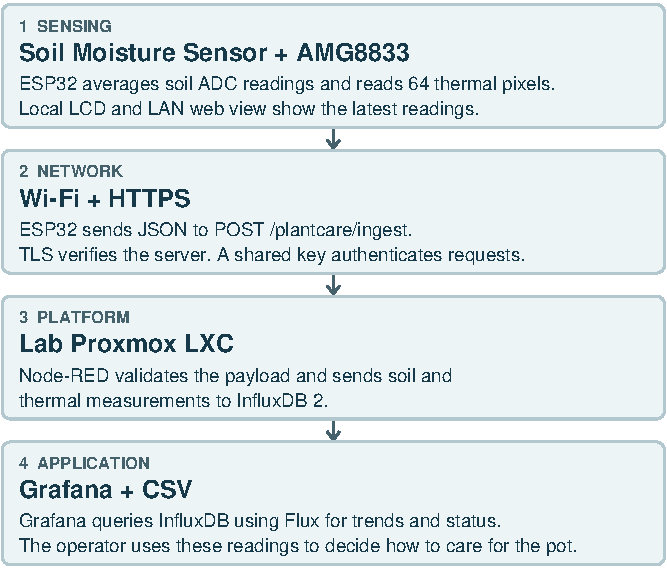
\includegraphics[width=.96\columnwidth]{architecture.pdf}
\caption{PlantCare telemetry flows from the sensing device through HTTPS to the lab platform and its user-facing outputs. The ESP32 also provides a direct LCD and local HTTP view.}
\label{fig:architecture}
\end{figure}

\begin{table}[!t]
\caption{Technology mapping for the implemented architecture.}
\label{tab:layers}
\centering\footnotesize
\begin{tabular}{@{}L{.18\columnwidth}L{.29\columnwidth}L{.45\columnwidth}@{}}
\hline
Layer & Technology & Function\\ \hline
Sensing & ESP32, probe, AMG8833, LCD1602 & Local two-second sensing, ADC smoothing, thermal view and device display.\\
Network & Wi-Fi, HTTPS, JSON & Sends the latest valid sections about once per minute.\\
Platform & Lab Proxmox LXC, Node-RED, InfluxDB 2 & Ingest, field shaping and time-series persistence.\\
Application & Grafana and CSV workflow & Current readings, status, trends, and offline review of exported records.\\ \hline
\end{tabular}
\end{table}

\emph{Sensing.} The capacitive probe supplies an analog value from one position in the pot. The AMG8833 reads 64 infrared pixel temperatures over I$^2$C. The ESP32 maintains a recent snapshot for all its outputs, so serving a local request does not trigger a second measurement.

\emph{Network.} The ESP32 sends JSON via Wi-Fi over a TLS connection with server certificate validation. The JSON carries identifiers and optional sensor objects so the server can associate readings even when only one sensor is available.

\emph{Platform.} Node-RED is the ingestion and shaping service. InfluxDB stores the resulting timestamped fields. The project identifies the deployment as lab-hosted Proxmox LXC. The reviewed flow targets InfluxDB 2 using the Node-RED InfluxDB integration. The deployment inventory was unavailable, so the report describes the service boundaries without assigning individual services to specific containers.

\emph{Application.} Grafana reads InfluxDB through the PlantcareIOT data source. Current readings, freshness, trends, and historical rows serve different purposes. An export allows review outside Grafana and can preserve selected history beyond the database retention period if archived independently. The application leaves the plant owner in control.

\begin{table}[!t]
\caption{Changes from the original proposal and their consequences.}
\label{tab:changes}
\centering\footnotesize
\begin{tabular}{@{}L{.27\columnwidth}L{.31\columnwidth}L{.34\columnwidth}@{}}
\hline
Proposal & Implemented or reported & Rationale and trade-off\\ \hline
AWS EC2 services, S3 archive & Lab Proxmox LXC, InfluxDB, Grafana, reported daily CSV export & Reuses the lab stack and makes data review straightforward. Archive durability depends on where files are stored.\\
Mosquitto with MQTT/TLS QoS 1 & Direct HTTPS POST to Node-RED & One request contract for a periodic snapshot. New TLS connections add overhead.\\
JWT registration and assigned topic prefix & Configured endpoint and static header key & Simpler provisioning for one device, with less granular credential management.\\
Thermal summary at the ESP32 and a replay buffer & Full valid frame on upload, local min/max and local heatmap & Retains spatial detail for server processing. Missed periods can leave permanent history gaps.\\
Approximate soil moisture classes and recommendations & Relative index, current values and trial status in Grafana & Makes thresholds traceable to one trial and keeps care decisions manual.\\ \hline
\end{tabular}
\end{table}

The MQTT test flow documents the earlier broker experiment. The rationale in Table~\ref{tab:changes} describes engineering fit inferred from the artifacts.

\subsection{MQTT Topic Hierarchy}
The proposal organized MQTT routing as \path{plantcare/site/plant/device/type}. Its worked example was \path{plantcare/ait/plant01/esp32_01/soil}, with a project namespace, site, plant, device, and stream. The production-style HTTPS client uses one route and carries the plant and device identifiers in the request body, with soil and thermal sections selecting the stream. The bucket separates those streams by measurement, while tags enable filtering by identity and data source. The proposed site level has no corresponding field in the observed firmware payload. The exported Node-RED flow subscribes to \path{plantcare/ait/plant01/esp32_01/+} and routes messages to a debug node. The \code{soil}, \code{thermal}, and \code{status} topics exercise a separate validation path. The live sensor write path shown in Fig.~\ref{fig:nodered} uses HTTPS.

\subsection{REST API Contract}
The firmware calls \code{POST /plantcare/ingest} over HTTPS. The host and key are omitted. The required content type is \code{application/json}. The caller sends the shared key in \code{x-plantcare-key}. An illustrative soil-only body using the verified field names is:

{\footnotesize
\begin{verbatim}
{
  "plant_id": "plant01",
  "device_id": "esp32_01",
  "data_source": "real",
  "soil": {
    "sensor_ok": true, "raw": 2468,
    "filtered_raw": 2466,
    "relative_wetness_pct": 43.53
  }
}
\end{verbatim}
}
The thermal object, when present, contains \code{pixels}, an ordered array of 64 temperatures in degrees Celsius. The firmware skips a request if neither sensor is ready. It treats \code{202 Accepted} as successful ingestion for downstream processing. The exported handler returns the following JSON on acceptance (soil-only example).
{\footnotesize
\begin{verbatim}
{"ok":true,"accepted":true,
 "soil":true,"thermal":false}
\end{verbatim}
}
A missing or invalid key returns \code{401} with \code{invalid\_api\_key}. Malformed or invalid telemetry returns \code{400} and an error code, such as \code{invalid\_json} or \code{invalid\_thermal}. A request with neither sensor returns \code{no\_sensor\_data}. On rejection the handler emits no database messages.

\section{Research Methodology and Implementation}
\subsection{Device-Level Stack}
Figure~\ref{fig:hardware} shows the ESP32 development kit, LCD, cabling, and hanging pot. The firmware uses Arduino C/C++, the ESP32 Wi-Fi and web-server libraries, and the Adafruit AMG88xx library. The probe is read on GPIO34 (ADC1), with a 12-bit ADC configuration. The I$^2$C bus uses GPIO21 and GPIO22. The board is shown cabled during operation. Supply voltage at the probe, operating current, and power were not measured in the retained evidence.

\begin{figure*}[!t]
\centering
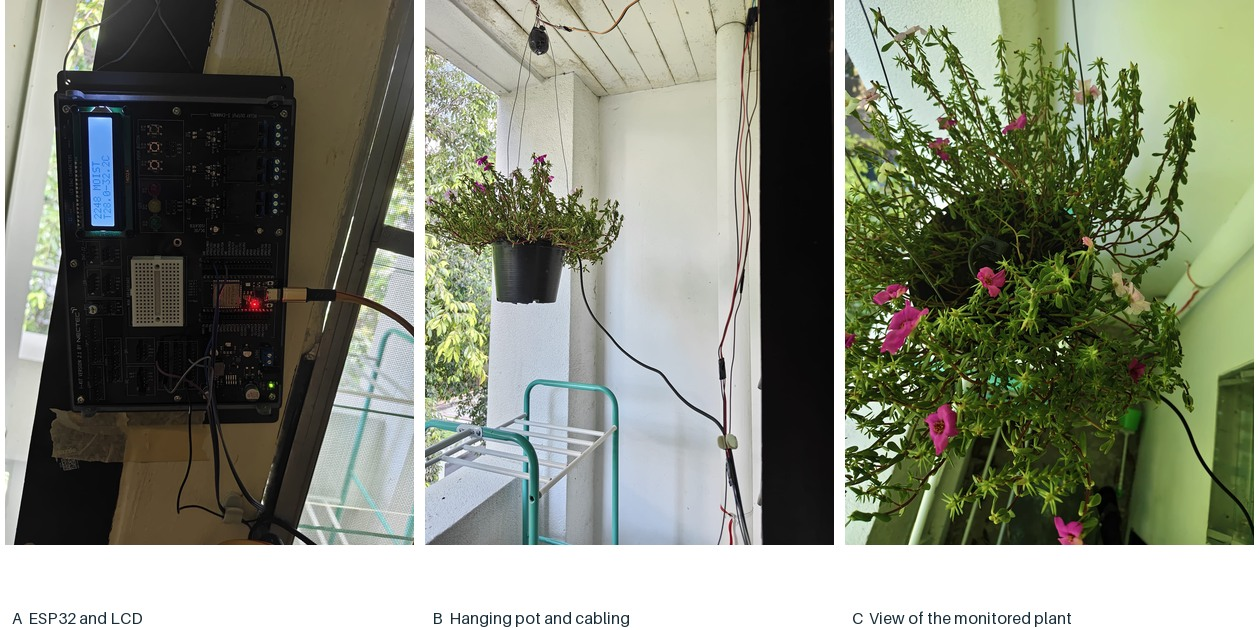
\includegraphics[width=.67\textwidth]{hardware.jpg}
\caption{PlantCare field setup. (A) ESP32 development kit and illuminated LCD. (B) Hanging pot and cable routing near the balcony opening. (C) Close view of the monitored plant. Source: local project photographs.}
\label{fig:hardware}
\end{figure*}

The sketch averages 20 ADC reads, spaced by approximately 3 ms in the loop. It excludes means at or below 10 or at or above 4085 as a basic plausibility check. The exponential moving average (EMA) uses weight 0.25 for the latest valid mean and 0.75 for the previous estimate. On initialization or after an invalid sample, the next valid sample seeds the filter. The calculation clips the relative wetness index to the observed scale:
\begin{equation}
W=\operatorname{clip}_{[0,100]}\!
   \left(100\,\frac{2614-A_{\rm EMA}}{2614-2274}\right).
\label{eq:wetness}
\end{equation}
Here $A_{\rm EMA}$ is in ADC counts. The archived sketch implements the mapping below, excerpted with comments omitted. The recorded raw field is the 20-read mean.
{\footnotesize
\begin{verbatim}
float index =
  (SOIL_BEFORE_WATER_REF - currentADC) /
  referenceRange * 100.0f;
return constrain(index, 0.0f, 100.0f);
\end{verbatim}
}
The endpoints refer to the average before watering and immediately after watering. They do not establish physically dry or saturated soil. Clipping hides variation beyond the endpoints in $W$, so retaining raw and filtered ADC values matters. The EMA also delays the index response to sudden changes. Invalid soil is represented as unavailable in the local JSON and omitted in the HTTPS body.

For thermal data, the sketch checks I$^2$C connectivity and finite pixel values, calculates the frame minimum and maximum, and updates the cached frame. The local browser interpolates the image for display from 64 measured cells. Interpolation adds no new spatial information. A pixel can include foliage, pot, wall, or background. Sensor orientation, distance, and surface emissivity therefore limit interpretation. Node-RED splits each row into columns 0--3 and 4--7 using the pixel index modulo eight. It averages the 32 values in each half and writes the absolute difference $\Delta T=|T_{\rm left}-T_{\rm right}|$ alongside the frame minimum and maximum. The left and right labels describe array coordinates. Their physical orientation depends on how the sensor was mounted.

\subsection{Platform Containerization}
The lab platform runs the server-side services on Proxmox LXC. Node-RED accepts telemetry and emits separate InfluxDB messages for valid soil and thermal sections. The flow uses \code{node-red-contrib-influxdb} version 0.7.0 and targets an InfluxDB 2 bucket named \code{plantcare}. Grafana reads it over a Flux data source. The InfluxDB integration uses millisecond write precision in the exported configuration. Figure~\ref{fig:nodered} shows the three outputs of the ingest function \cite{projectevidence}. The adjacent MQTT debug, simulated validation, and manual write tests have distinct purposes. Grafana filters for \code{data\_source=real} to exclude simulated writes.

\begin{figure*}[!t]
\centering
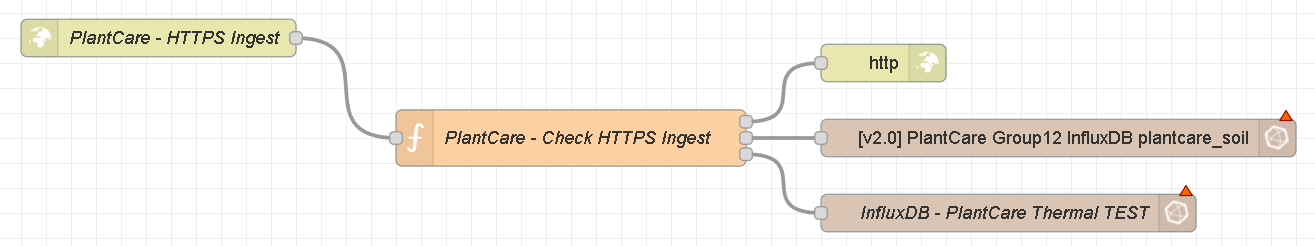
\includegraphics[width=.84\textwidth]{node-red-ingest.png}
\caption{HTTPS ingest branch of the Node-RED editor. The validator sends a response on its first output and routes accepted soil and thermal records to separate InfluxDB nodes. The crop excludes the connection settings sidebar.}
\label{fig:nodered}
\end{figure*}

The recorded schema pairs \code{plantcare\_soil} with \code{soil\_adc\_raw}, \code{soil\_adc\_filtered}, and \code{relative\_wetness\_pct}. The thermal measurement \code{plantcare\_thermal} has \code{t\_min\_c}, \code{t\_max\_c}, \code{t\_left\_c}, \code{t\_right\_c}, and \code{delta\_t\_c}. Historical query context identifies tags \code{plant\_id}, \code{device\_id}, and \code{data\_source}. The submitted JSON body lacks an explicit acquisition timestamp. A stored time or a Grafana minute label consequently cannot be used as a device-to-dashboard latency measurement.

\emph{Retention and scheduled export.} The reported configuration for \code{plantcare} is 180 days (4,320 hours). InfluxDB's retention service removes eligible shard groups after their time range ages out \cite{retention}. The project reports a daily Cron job that exports historical data to CSV. The schedule time, timezone, script, output location, raw execution log, and counts from the scheduled files remain unverified. CSV retention is a separate operational policy. Local CSV copies support analysis, while a recoverable backup requires a separately retained and tested copy. The following read-only checks are for the authorized lab operator using the active Influx CLI configuration and the job owner's account. Their outputs are pending.
{\footnotesize
\begin{verbatim}
influx bucket list --name plantcare
crontab -l
\end{verbatim}
}

\subsection{Identity and Access Management}
The ESP32 waits for plausible wall-clock time before attempting TLS and configures a CA root with \code{setCACert}. The request carries a shared key. The Node-RED function reads its expected value from \code{PLANTCARE\_INGEST\_KEY} and rejects requests when the key is absent, too short, or different from the configured value. The firmware excerpt shows the client side of the exchange.
\begin{minipage}{\columnwidth}{\footnotesize
\begin{verbatim}
client.setCACert(CLOUD_ROOT_CA);
// ... connection setup ...
https.addHeader("Content-Type",
                "application/json");
https.addHeader("x-plantcare-key",
                CLOUD_API_KEY);
const int status = https.POST(payload);
\end{verbatim}
}\end{minipage}
TLS validates the server, while the shared key is the device-side credential. The visible \code{device\_id} is a payload identifier. The inspected sketch uses a static key provisioned with firmware, with no rotation, TTL, or refresh exchange. The ESP32's local HTTP routes are a separate LAN-only access assumption and the code does not enforce route-level authentication. The exported flow configures an internal HTTP hop to InfluxDB. Restrict that hop to the lab network or use TLS across an untrusted network. The artifacts establish the ESP32 HTTPS boundary and the ingest check. They do not establish token scopes, Grafana roles, or network exposure. For a larger deployment, per-device provisioning, scoped service tokens, and secret-free source distribution would make credential compromise easier to contain.

\subsection{End-to-End Data Flow}
\begin{enumerate}
\item The ESP32 reads the probe and the AMG8833 on a nominal two-second schedule. It averages and filters soil ADC values, normalizes the result, and validates the thermal frame.
\item The LCD, Serial Monitor, and local web view read the cached snapshot. The browser can fetch \code{/soil} and \code{/thermal}; the latter returns \code{503} when the thermal frame is unavailable.
\item At the upload interval the ESP32 checks Wi-Fi, clock, key configuration, and sensor readiness. It POSTs the latest valid sections. A missed attempt leaves no replay record in the inspected sketch.
\item Node-RED accepts the snapshot and shapes the data for InfluxDB. The schema and output fragment show measurement-based storage. Query results provide separate evidence of storage.
\item Grafana reads the historical series and current values. A separate CSV path supports offline review. The plant owner may then inspect the pot and make a manual intervention.
\end{enumerate}
\section{Experimental Evaluation and Results}
\begin{figure*}[!t]
\centering
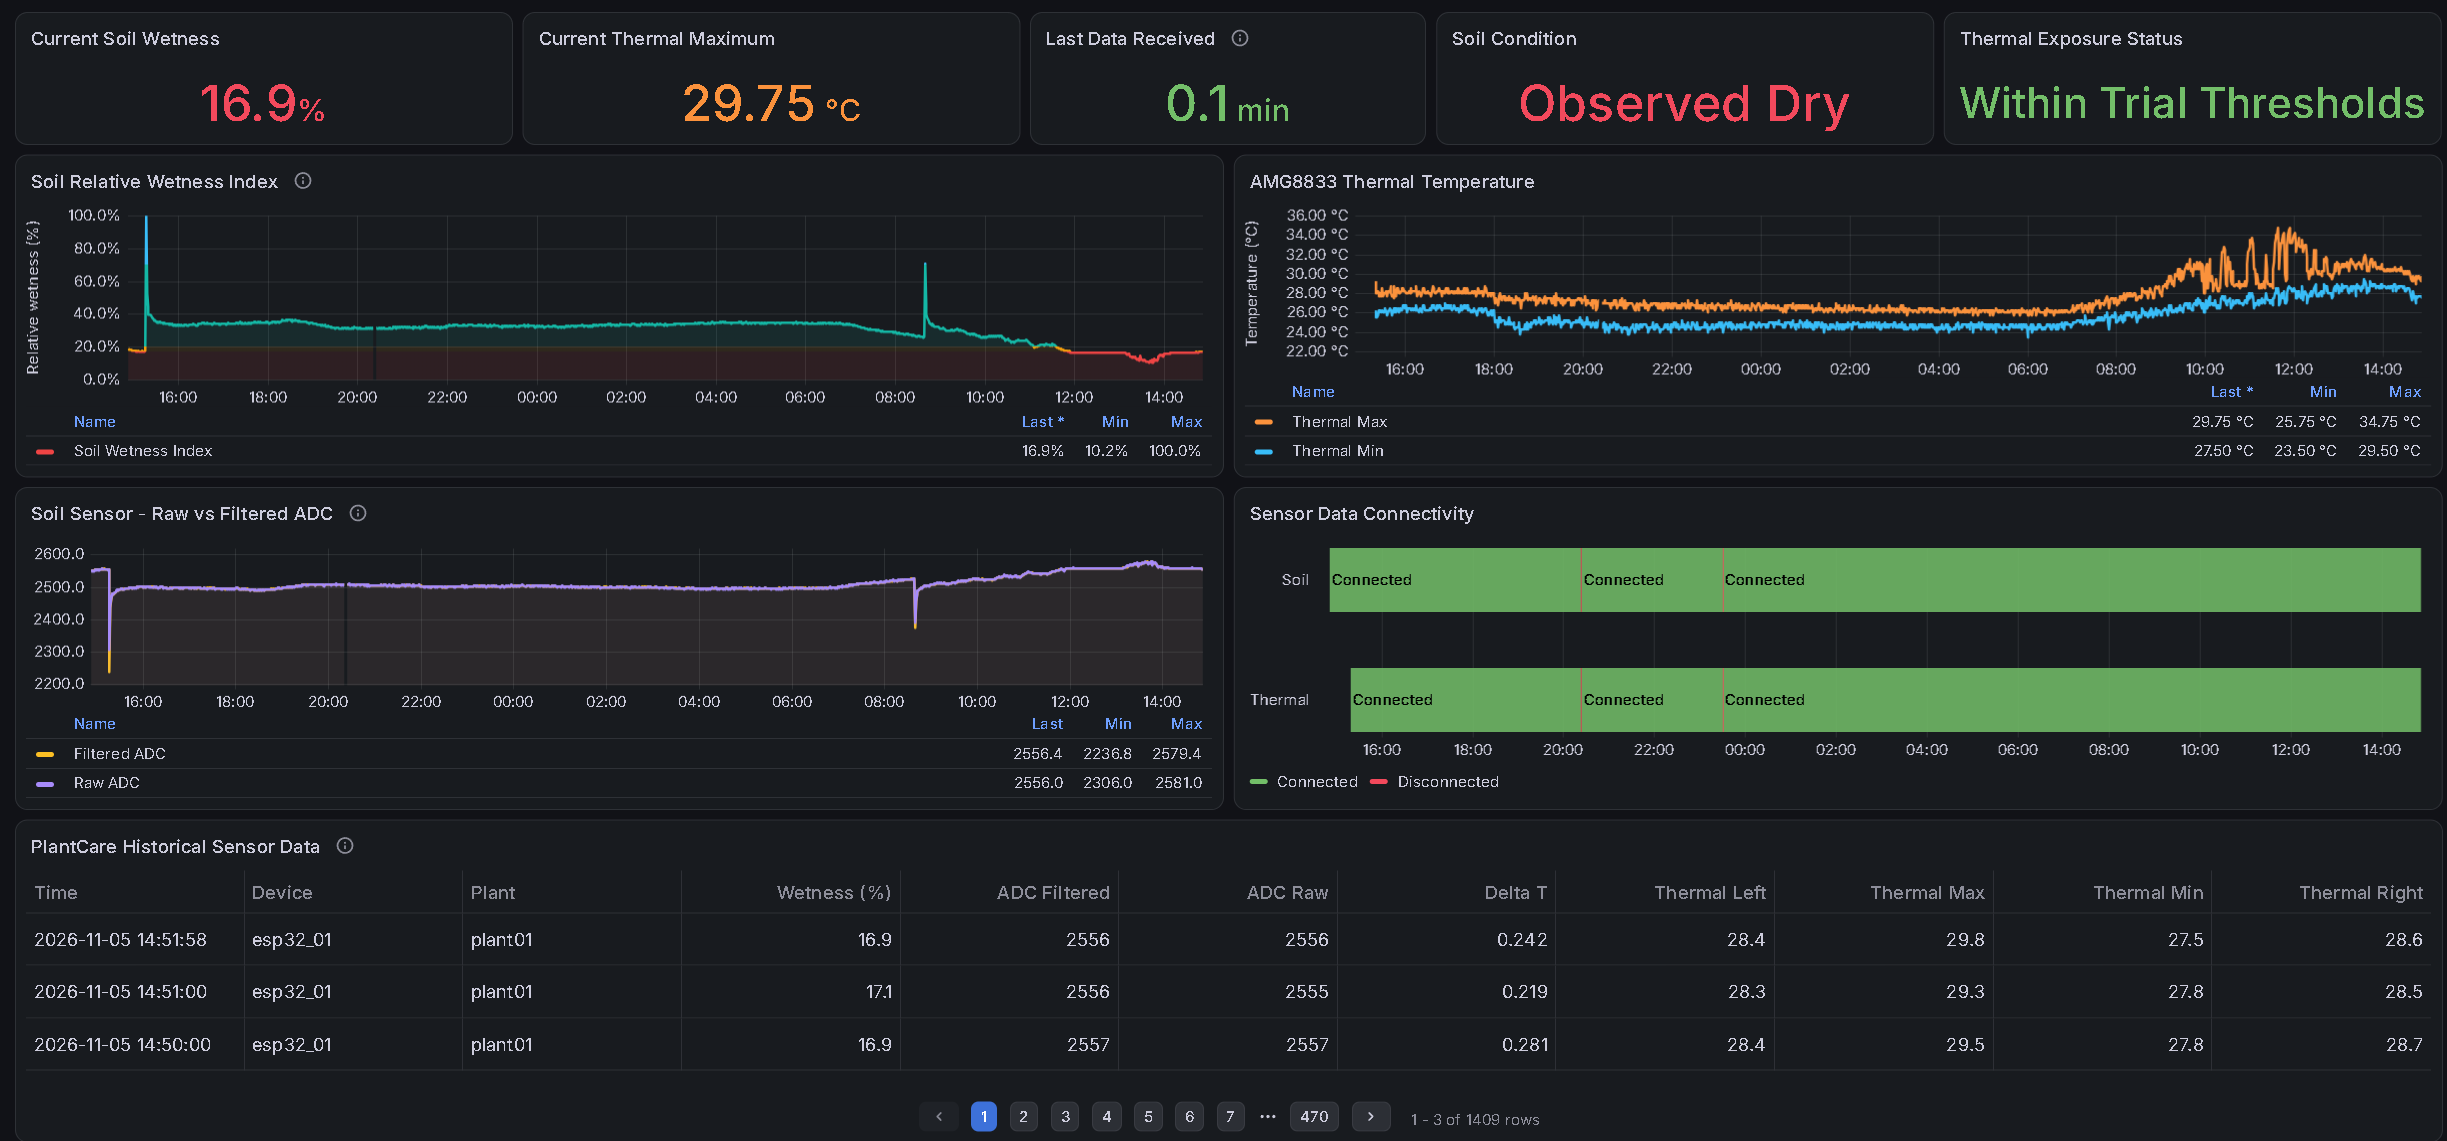
\includegraphics[width=.86\textwidth]{grafana.png}
\caption{Updated Grafana capture from 5 November 2026 showing current readings, both status cards, sensor timelines, and historical rows. The crop removes the browser address and controls.}
\label{fig:grafana}
\end{figure*}
\subsection{Trial Setup and Observed Soil Response}
The observational trial used one hanging pot and the photographed thermal viewing arrangement. The assessment combines before/after snapshots from the ESP32 dashboard, firmware and flow artifacts, a saved Grafana Explore export, and dashboard captures \cite{projectevidence}. The historical export represents one device and plant. The record audit uses the timestamps as printed because the CSV has no UTC offset. Network conditions, power interruptions, and server load were not instrumented.

The exported ingest function passed eight offline checks using a synthetic key and fixture payloads. Soil-only and combined requests returned \code{202}. Invalid key, malformed JSON, wrong device, out-of-range ADC, short thermal frame, and empty sensor payload returned their expected errors and emitted no write messages. The combined fixture used half-frame means of $26\degc$ and $29\degc$ and returned $\Delta T=3\degc$. This exercise covered function behavior without making network requests or measuring write reliability.

Table~\ref{tab:watering} shows four paired observations. The paired mean ADC fell from 2,614 to 2,273.5, a difference of 340.5 counts. The firmware rounds the wet endpoint to 2,274. Every immediate post-watering value is lower than its paired initial value. In the 20 October sequence the reading subsequently rose to 2,501 at 18:24 and 2,522 at 18:57. The sequence supports a short-term sensor response in this pot. The observations lack controlled water volumes, a reference moisture measurement, and independent replicate pots.

\begin{table}[!t]
\caption{Raw ADC before and immediately after manual watering, transcribed from local dashboard captures.}
\label{tab:watering}
\centering\footnotesize
\begin{tabular}{@{}lrrr@{}}
\hline
Observation & Before & After & Drop\\ \hline
20 Oct., evening & 2770 & 2307 & 463\\
21 Oct., morning & 2622 & 2238 & 384\\
21 Oct., evening & 2559 & 2226 & 333\\
22 Oct., morning & 2505 & 2323 & 182\\ \hline
Mean & 2614 & 2273.5 & 340.5\\ \hline
\end{tabular}
\end{table}

\subsection{CSV Completeness and Data Gaps}
The Grafana Explore file saved on 3 November 2026 covers displayed timestamps from 29 October at 09:54 through 3 November at 17:00. A CSV parser counted 5,860 data rows after the header and found 5,860 distinct timestamp, device, and plant keys. All rows have the three soil fields. Of these, 5,844 have all five thermal fields and 16 lack all thermal fields. Thus 99.7\% of exported rows contain both measurement families. A pivoted table row can combine multiple fields and measurements at one minute. Raw InfluxDB points and scheduled archive rows must be counted separately. The Explore CSV has no data-source tag column.

\begin{table}[!t]
\caption{Recounted Grafana Explore rows by displayed date. The first and last dates are partial.}
\label{tab:daily}
\centering\footnotesize
\begin{tabular}{@{}lrrr@{}}
\hline
Date in 2026 & Rows & With soil & With thermal\\ \hline
29 Oct. & 823 & 823 & 823\\
30 Oct. & 1369 & 1369 & 1369\\
31 Oct. & 1340 & 1340 & 1340\\
1 Nov. & 872 & 872 & 872\\
2 Nov. & 1396 & 1396 & 1380\\
3 Nov. & 60 & 60 & 60\\ \hline
Total & 5860 & 5860 & 5844\\ \hline
\end{tabular}
\end{table}

Comparing adjacent timestamps found 141 separations longer than one minute. The largest were 967 minutes (2 November at 23:52 to 3 November at 15:59), 581 minutes (31 October at 23:05 to 1 November at 08:46), and 34 minutes (30 October at 13:05 to 13:39). Across the inclusive export span, 5,860 of 7,627 nominal minute slots appear (76.8\%). The 1,767 absent slots describe this file's coverage. Device downtime, Wi-Fi or TLS failure, ingestion failure, or export query behavior could each produce missing rows. Attribution requires correlated timestamps from firmware, ingest, and database logs.

\subsection{Grafana Visualization and Status Thresholds}
Figure~\ref{fig:grafana} shows a soil index of 16.9\%, a thermal maximum of $29.75\degc$, and a latest soil reading age of about 0.1 min. The two cards show Observed Dry and Within Trial Thresholds. The historical table shows 1,409 rows for the dashboard selection at capture. That selection is separate from the 5,860-row Explore export. The connectivity query marks a missing-data interval after a 180-second gap. This indicates absent telemetry and does not directly measure Wi-Fi connectivity.

The soil trial uses four display bands. The boundaries at 17, 20, and 70\% reflect the team's observations of low readings before watering, short peaks after watering, and subsequent settling. Grafana Stat value mappings render those bands as labels \cite{grafana}. The current maximum panel uses orange below $35\degc$ and red from $35\degc$. The exported numeric tiles query the previous 15 minutes. Both status cards use a three-minute window, and thermal status requires a recent pair at the same timestamp. Table~\ref{tab:thresholds} lists the saved rule boundaries, with the elevated maximum taking priority.

\begin{table}[!t]
\caption{Experimental dashboard rules. Wetness is a relative index. The thermal rules are evaluated top to bottom.}
\label{tab:thresholds}
\centering\footnotesize
\begin{tabular}{@{}L{.41\columnwidth}L{.53\columnwidth}@{}}
\hline
Reading & Trial label and color\\ \hline
$W<17\%$ & Observed Dry (red)\\
$17\%\leq W<20\%$ & Low Wetness (amber)\\
$20\%\leq W<70\%$ & Observed Moderate (teal)\\
$W\geq70\%$ & High Wetness Reading (blue)\\ \hline
$T_{\max}\geq35\degc$ & Elevated Temperature (red)\\
$\Delta T\geq2\degc$ with $T_{\max}<35\degc$ & Uneven Thermal Exposure (amber)\\
Both below thresholds & Within Trial Thresholds (green)\\
No recent complete input & No recent data\\ \hline
\end{tabular}
\end{table}

During panel editing, the generic InfluxDB source produced a bucket error. The updated capture shows both status cards populated. The export includes a data-source selector, while the panel queries retain a fixed InfluxDB data-source identifier. A new deployment must rebind those queries to its own source. Its no-value text is \emph{No recent data}, and the saved status panels have a green base threshold. Interpret the text and freshness before relying on color. A bucket error and a successful query with no recent points require different diagnosis.

Offline application of the saved bands assigns 4,203 soil rows to Observed Dry, 35 to Low Wetness, 1,621 to Observed Moderate, and 1 to High Wetness Reading. The 5,844 complete thermal rows have a maximum-temperature range of $22.8$ to $34.5\degc$ and a recorded difference from $0$ to $1.31\degc$. They all fall below the thermal rule boundaries. Controlled tests are needed for the elevated and uneven thermal states. Validating plant-health interpretations would also require independent observations.

\subsection{Cloud-Only Baseline and Required Benchmarks}
Table~\ref{tab:bench} records the remaining course measurements. The proposed control is a cloud VM running equivalent ingest, persistence, and dashboard logic for the same replayed sensor sequence, with filtering and presentation shifted to the remote service. First hold rate, payload, and protocol constant to isolate placement. Then vary the sampling-to-upload ratio or compare MQTT over TLS with HTTPS using the same payload and delivery accounting. Repeat on a normal link and under a defined impairment, for example 100 ms added round-trip delay and 1\% packet loss. Record actual settings, repetitions, and hardware resources.

\begin{table}[!t]
\caption{Required quantitative evaluation and current evidence status.}
\label{tab:bench}
\centering\footnotesize
\begin{tabular}{@{}L{.35\columnwidth}L{.60\columnwidth}@{}}
\hline
Measurement & Method and status\\ \hline
Gateway and VM CPU/memory & \code{sysbench} CPU events/s and memory MiB/s. No paired host measurements.\\
Database disk I/O & \code{dd} read/write throughput on an isolated test volume (MiB/s). Unmeasured.\\
Link capacity and loss & \code{iperf3} TCP throughput and UDP loss/jitter under the same link profile \cite{iperf}. Unmeasured.\\
Latency & Report p50 and p95 in ms from a timestamped input to durable query visibility. Unmeasured.\\
Bandwidth savings & Capture HTTPS and MQTT bytes per delivered sample, including handshakes and retries. Unmeasured.\\
Power efficiency & Integrate measured supply power over a fixed trial and divide by delivered samples (J/sample). Unmeasured.\\ \hline
\end{tabular}
\end{table}

\code{iperf3} characterizes the link, and captures from the two application paths quantify protocol overhead. Log timestamps at source, acceptance, persistence, and query visibility so that HTTP acceptance and dashboard refresh can be analyzed separately. Compare aggregate bytes for equal-duration trials with the same source workload, and report delivery completeness alongside any savings. The available evidence supports an observational evaluation only. The cloud-only comparison requires a separate benchmark run.

\section{Conclusion and Future Work}
PlantCare integrates two physical sensing channels with local feedback, periodic HTTPS telemetry, lab-hosted time-series storage, and a Grafana view. The watering observations support a relative soil response, and the reviewed export establishes the amount and continuity of the available history. The deployed approach retains the proposal's manual decision loop and replaces the MQTT and AWS path with a simpler lab workflow. Certificate validation protects the uplink trust boundary and the static device key limits how credentials can be managed. Long gaps and partial thermal rows matter when interpreting recent status. The prototype supports monitoring and inspection for one pot. Its effects on water use, thermal stress, uptime, and energy efficiency remain unmeasured.

The next experiment should pair repeated, measured watering events across multiple pots with an independent moisture reference. Record sensor placement, water volume, and timestamps, and deliberately test loss and recovery on an isolated link. This would separate substrate and sensor effects from network gaps and provide the observations needed to revise the display thresholds.


\begin{thebibliography}{00}
\bibitem{fao} Food and Agriculture Organization of the United Nations, \emph{Water Use Methodology}, AQUASTAT. [Online]. Available: \url{https://www.fao.org/aquastat/en/overview/methodology/water-use/index.html}
\bibitem{calibration} A. A. Abdelmoneim, C. M. Al Kalaany, R. Khadra, B. Derardja, and G. Dragonetti, “Calibration of low-cost capacitive soil moisture sensors for irrigation management applications,” \emph{Sensors}, vol. 25, no. 2, Art. no. 343, 2025, doi: 10.3390/s25020343.
\bibitem{iira} Industry IoT Consortium, \emph{The Industrial Internet Reference Architecture}, ver. 1.10, Nov. 2022. [Online]. Available: \url{https://www.iiconsortium.org/wp-content/uploads/sites/2/2022/11/IIRA-v1.10.pdf}
\bibitem{mqtt} OASIS, \emph{MQTT Version 5.0}, OASIS Standard, Mar. 2019. [Online]. Available: \url{https://docs.oasis-open.org/mqtt/mqtt/v5.0/os/mqtt-v5.0-os.html}
\bibitem{http} R. Fielding, M. Nottingham, and J. Reschke, Eds., \emph{HTTP Semantics}, RFC 9110, Jun. 2022, doi: 10.17487/RFC9110.
\bibitem{kim} Y. Kim, R. G. Evans, and W. M. Iversen, “Remote sensing and control of an irrigation system using a distributed wireless sensor network,” \emph{IEEE Trans. Instrum. Meas.}, vol. 57, no. 7, pp. 1379--1387, Jul. 2008, doi: 10.1109/TIM.2008.917198.
\bibitem{tensiometer} A. A. Abdelmoneim, R. Khadra, B. Derardja, and G. Dragonetti, “Internet of Things (IoT) for soil moisture tensiometer automation,” \emph{Micromachines}, vol. 14, no. 2, Art. no. 263, 2023, doi: 10.3390/mi14020263.
\bibitem{proposal} J. Datephanyawat and W. Neamtuptim, “PlantCare IoT: An edge--cloud soil moisture and thermal exposure monitoring system for potted plants,” AST01.41 interim project proposal, Asian Institute of Technology, 2026, unpublished.
\bibitem{projectevidence} PlantCare IoT project team, Arduino sketch, Node-RED flow export, local watering screenshots, Grafana dashboard JSON and screenshots, and Grafana Explore CSV saved Nov. 3, 2026, unpublished project artifacts, 2026.
\bibitem{retention} InfluxData, \emph{Data Retention in InfluxDB}, InfluxDB OSS v2 Documentation. [Online]. Available: \url{https://docs.influxdata.com/influxdb/v2/reference/internals/data-retention/}
\bibitem{grafana} Grafana Labs, \emph{Configure Value Mappings}, Grafana Documentation. [Online]. Available: \url{https://grafana.com/docs/grafana/latest/visualizations/panels-visualizations/configure-value-mappings/}
\bibitem{iperf} Energy Sciences Network, \emph{Invoking iperf3}, iperf3 Documentation. [Online]. Available: \url{https://software.es.net/iperf/invoking.html}
\end{thebibliography}


\EOD
\end{document}

